% =====================================================================
%  Fundamentals of Deep Learning — Class 2
%  Topic: Introduction to Neural Networks
%  Biology and the brain; McCulloch-Pitts neuron; thresholding and
%  linear separability.
%
%  Plots are produced by  src/make_figures.py  (SciencePlots "science"
%  preset, Fira Sans).  Concepts follow Rojas (1996), Ch. 1-2.
%
%  Compile:  xelatex main.tex   (run twice)
% =====================================================================
\documentclass[aspectratio=169, 11pt]{beamer}

\usetheme{metropoliscustom}

\usepackage{graphicx}
\DeclareGraphicsExtensions{.pdf,.png,.jpg}  % prefer vector PDF
\graphicspath{{figs/}{Class02_Intro_Neural_Networks/B_Recreated_Figures/figs/}}
\usepackage{amsmath, amssymb}
\usepackage{bm}
\usepackage{tikz}
\usetikzlibrary{arrows.meta, positioning, calc, decorations.pathreplacing,
                backgrounds, fit}
\tcbuselibrary{skins}

% ---- shared palette -------------------------------------------------
\definecolor{shc}{HTML}{341651}    % inputs / biology side
\definecolor{tealc}{HTML}{1C7293}  % activations
\definecolor{dpc}{HTML}{800000}    % output / model side
\definecolor{accc}{HTML}{B8860B}   % fourth series

% ---- parallel strip: Biology (left) vs Model (right)
\newcommand{\biomodel}[2]{%
  \vfill
  {\footnotesize
  \begin{tcolorbox}[enhanced, sidebyside, sidebyside align=top,
                    lefthand ratio=0.485,
                    segmentation style={shc!35, line width=0.6pt},
                    colback=shc!5, colframe=shc!35, boxrule=0.5pt,
                    arc=1.5mm, left=2mm, right=2mm, top=0.8mm, bottom=0.8mm]
    {\color{shc}\textbf{BIO}}\;\; #1
  \tcblower
    {\color{dpc}\textbf{MODEL}}\;\; #2
  \end{tcolorbox}}%
  \vspace{0.6em}%
}

\newcommand{\figsource}[1]{{\scriptsize\color{mcMuted} #1}}

% ---- a unit drawn as a circle with its activation inside ------------
% #1 name  #2 position  #3 colour  #4 label (placed above)
\newcommand{\unit}[4]{%
  \node[circle, draw=#3, fill=#3!6, line width=1.0pt,
        minimum size=16mm, inner sep=0pt] (#1) at #2 {};
  \begin{scope}
    \clip #2 circle (0.8);
    \draw[tealc, line width=1.6pt]
      ($#2+(-0.80,-0.42)$) -- ($#2+(0.03,-0.42)$) -- ($#2+(0.74,0.45)$);
  \end{scope}
  \node[font=\large, #3] at ($#2+(0,1.12)$) {#4};
}
\newcommand{\plainunit}[4]{%
  \node[circle, draw=#3, fill=black!4, line width=1.0pt,
        minimum size=16mm, inner sep=0pt, font=\normalsize]
        (#1) at #2 {#4};
}

% =====================================================================
\title{Introduction to Neural Networks}
\subtitle{Biology, the McCulloch--Pitts Neuron, and Linear Separability}
\author{Fundamentals of Deep Learning \ \textperiodcentered\ Class 2}
\institute{}
\date{28 July}

\footleft{DA3409 Deep Learning}
\footright{Introduction to Neural Networks}
\titlelogos{}

\begin{document}

\maketitle

\begin{frame}{Outline}
  \tableofcontents
\end{frame}

% =====================================================================
\section{The Biological Neuron}
% =====================================================================

\begin{frame}{The brain as an inspiration}
  \begin{itemize}
    \item The brain: roughly $10^{11}$ neurons, each connected
          to up to $10^{4}$ others --- massively
          \alert{parallel}, not sequential
    % \item Slow components ($\sim$ms switching) yet faster than
    %       any computer at perception and motor control
    \item Rojas: artificial neural networks are best understood
          as \alert{networks of primitive functions} ---
          simple units, wired together
          \hfill{\scriptsize Rojas (1996), \S1.3}
  \end{itemize}
  \vspace{0.4em}
  \begin{redhighlight}
    The plan: abstract the essential behaviour of a neuron
    into a simple computing unit, then study what networks of
    such units can do.
  \end{redhighlight}
\end{frame}

\begin{frame}{Anatomy of a neuron}
  \centering
  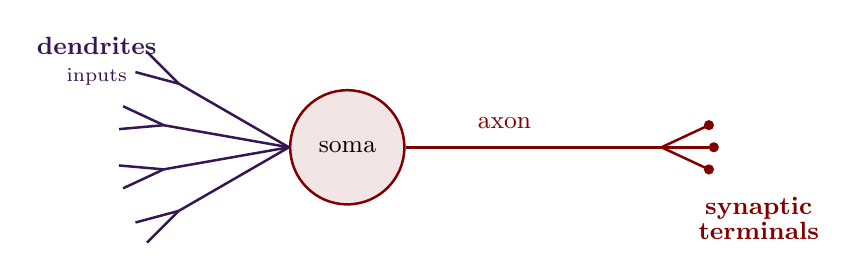
\begin{tikzpicture}[>=Stealth, line width=0.9pt, scale=0.95]
    \node[circle, draw=dpc, fill=dpc!10, minimum size=1.45cm]
      (soma) at (0,0) {\small soma};
    \foreach \a in {150,170,190,210}{
      \draw[shc] (soma.west) -- ++(\a:1.7);
      \draw[shc] ($(soma.west)+(\a:1.7)$) -- ++(\a+15:0.6);
      \draw[shc] ($(soma.west)+(\a:1.7)$) -- ++(\a-15:0.6);
    }
    \node[shc, align=center] at (-3.35,1.15)
      {\small\textbf{dendrites}\\[-2pt]{\scriptsize inputs}};
    \draw[dpc, line width=1.1pt] (soma.east) -- (4.2,0);
    \node[dpc] at (2.1,0.32) {\small axon};
    \foreach \a in {25,0,-25}{
      \draw[dpc] (4.2,0) -- ++(\a:0.7);
      \node[circle, fill=dpc, minimum size=2pt, inner sep=1.3pt]
        at ($(4.2,0)+(\a:0.7)$) {};
    }
    \node[dpc, align=center] at (5.5,-0.95)
      {\small\textbf{synaptic}\\[-3pt]\small\textbf{terminals}};
  \end{tikzpicture}
  \vspace{0.5em}
  \begin{itemize}\setlength{\itemsep}{1pt}
    \item \alert{Dendrites} collect incoming signals;
          the \alert{soma} integrates them
    \item If the integrated signal crosses a threshold, the
          neuron \alert{fires} an impulse down the \alert{axon}
    \item \alert{Synapses} pass the signal on --- some
          excitatory, some inhibitory
          \hfill{\scriptsize Rojas (1996), \S1.2}
  \end{itemize}
\end{frame}

\begin{frame}{Firing: an all-or-nothing threshold}
  \centering
  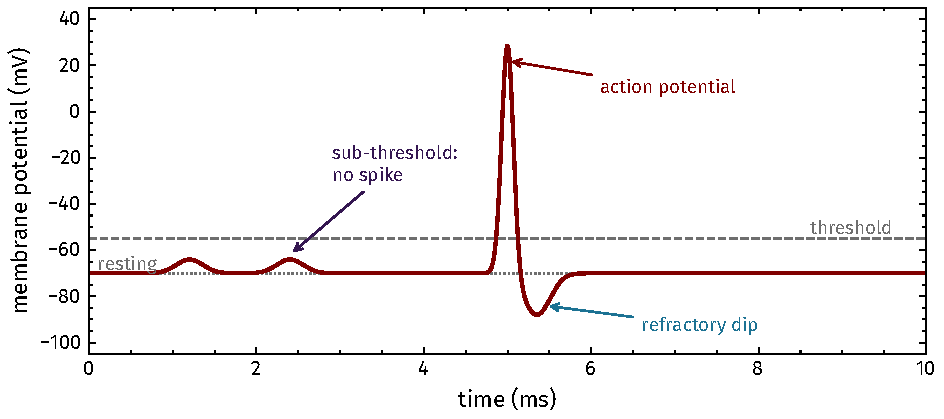
\includegraphics[height=0.40\textheight]{action_potential}
  \\[0.1em]
  \figsource{Membrane potential over time. Small inputs raise
  it but decay away; once it crosses the threshold the neuron
  emits a sharp, stereotyped \emph{action potential}, then dips
  below rest during the refractory period. The spike is
  \alert{all-or-nothing}: its shape encodes no magnitude ---
  only \emph{whether} and \emph{how often} the neuron fires.}
  \biomodel{potential crosses a threshold $\to$ spike}
           {weighted sum crosses a threshold $\to$ output $1$}
\end{frame}

\begin{frame}{At the synapse: adding and subtracting}
  \begin{itemize}
    \item Neurons meet at \alert{synapses}; a spike releases
          chemical messengers that nudge the next neuron
    \item \alert{Excitatory} synapses push the membrane
          \emph{toward} threshold; \alert{inhibitory} synapses
          push it \emph{away}
    \item The soma continuously \alert{sums} these pushes ---
          thousands of them --- and fires only if the net
          effect clears the threshold
    \item A single strong inhibitory input can \alert{veto}
          many excitatory ones
          \hfill{\scriptsize Rojas (1996), \S1.2.3}
  \end{itemize}
  \biomodel{excitatory $+$, inhibitory $-$, integrated at the
            soma}
           {positive and negative \alert{weights}, summed in
            the unit}
\end{frame}

% =====================================================================
\section{From Neuron to Computing Unit}
% =====================================================================

\begin{frame}{The abstract neuron}
  \begin{columns}[T, onlytextwidth]
    \begin{column}{0.50\textwidth}
      \centering
      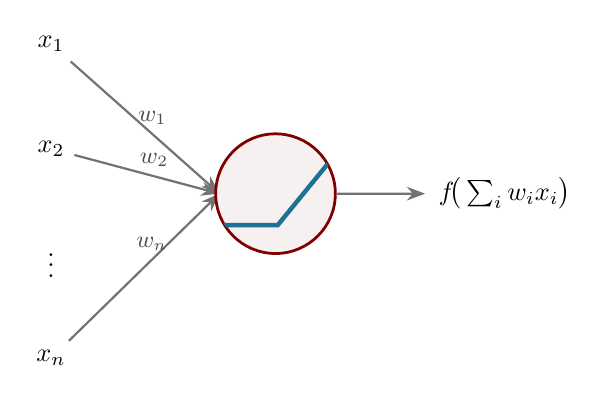
\begin{tikzpicture}[>=Stealth, line width=0.8pt,
          scale=0.95, transform shape, font=\normalsize]
        \foreach \i/\y in {1/2.1, 2/0.7, n/-2.1}{
          \node (x\i) at (0,\y) {$x_{\i}$};
          \draw[->, black!55] (x\i) -- node[above, pos=0.55,
            font=\small, black!70] {$w_{\i}$} (2.25,0.1);
        }
        \node at (0,-0.75) {$\vdots$};
        \unit{f}{(3.0,0.1)}{dpc}{}
        \draw[->, black!55] (f) -- (5.0,0.1);
        \node[right, font=\normalsize] at (5.05,0.1)
          {$f\!\big(\textstyle\sum_i w_i x_i\big)$};
      \end{tikzpicture}
    \end{column}
    \hfill
    \begin{column}{0.46\textwidth}
      \vspace{0.4em}
      \begin{itemize}\setlength{\itemsep}{2pt}
        \item Each input channel $i$ carries a value $x_i$,
              scaled by a \alert{weight} $w_i$
        \item The body integrates the inputs (usually a sum)
              and applies a \alert{primitive function} $f$
        % \item Everything in this course is a variation on this
        %       one picture
      \end{itemize}
    \end{column}
  \end{columns}
  \biomodel{dendrites $\times$ synaptic strengths, summed at
            the soma}
           {inputs $x_i$ $\times$ weights $w_i$, summed in the
            unit}
\end{frame}

\begin{frame}{Networks of primitive functions}
  \begin{itemize}
    \item An artificial neural network  can be visualized as a
          \alert{network of primitive functions}
          \hfill{\scriptsize Rojas (1996), \S1.3.1}
    \item Models differ only in three choices:
  \end{itemize}
  \vspace{0.4em}
  \centering
  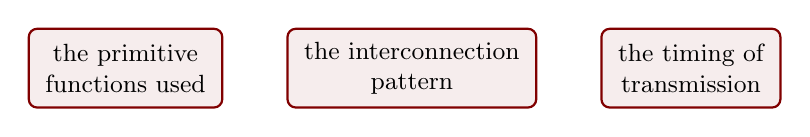
\begin{tikzpicture}[>=Stealth, line width=0.8pt, node distance=4mm,
      b/.style={rounded corners=3pt, draw=dpc, fill=dpc!7,
                align=center, minimum height=1.0cm,
                inner xsep=6pt, font=\small}]
    \node[b] (a) {the \alert{primitive}\\functions used};
    \node[b, right=8mm of a] (b) {the \alert{interconnection}\\pattern};
    \node[b, right=8mm of b] (c) {the \alert{timing} of\\transmission};
  \end{tikzpicture}
  \vspace{0.5em}
  \begin{itemize}
    \item Today's primitive function is the simplest possible
          --- a \alert{threshold}
  \end{itemize}
\end{frame}

\begin{frame}{Simple units add up to complicated functions}
  \centering
  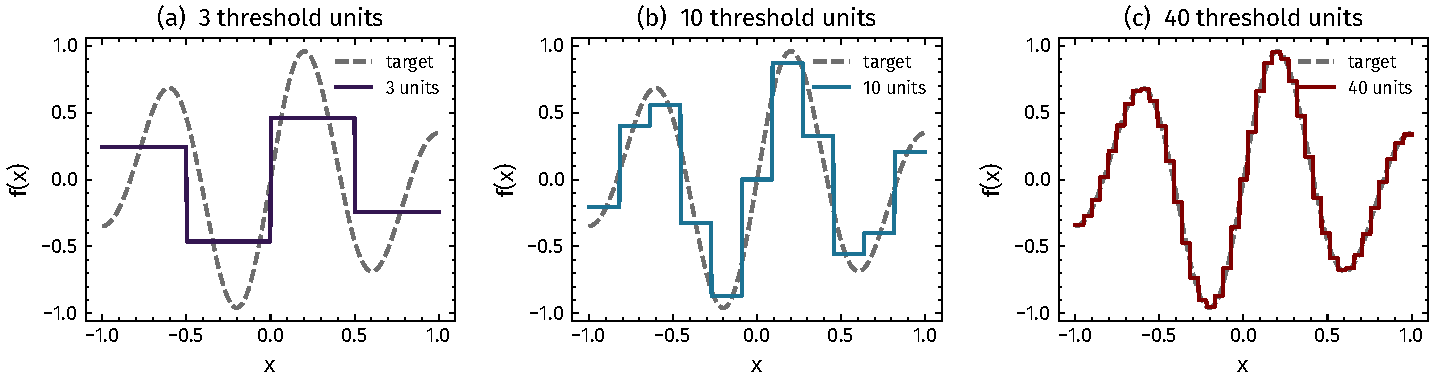
\includegraphics[height=0.36\textheight]{approximation}
  \\[0.15em]
  \figsource{Fitting $f(x)=\sin(2.4\pi x)\,e^{-x^2}$ (dashed)
  with a weighted sum of threshold units, each switching on at
  a different point. (a)~3 units, (b)~10, (c)~40 --- the
  staircase converges on the target as units are added.}
  \vspace{0.1em}
  \begin{itemize}\setlength{\itemsep}{0pt}
    \item Individually crude; \alert{summed}, they approximate
          anything --- this is a seed of universal function
          approximation 
  \end{itemize}
\end{frame}

\begin{frame}{Feed-forward vs.\ recurrent}
  \centering
  \begin{tikzpicture}[>=Stealth, line width=0.9pt,
      u/.style={circle, draw, minimum size=6mm, inner sep=0pt,
                font=\scriptsize}]
    \begin{scope}
      \node[u, draw=dpc, fill=dpc!8] (a1) at (0,0.6) {};
      \node[u, draw=dpc, fill=dpc!8] (a2) at (0,-0.6) {};
      \node[u, draw=dpc, fill=dpc!8] (b1) at (1.5,0) {};
      \node[u, draw=dpc, fill=dpc!8] (c1) at (3.0,0) {};
      \draw[->] (a1)--(b1); \draw[->] (a2)--(b1); \draw[->] (b1)--(c1);
      \node[font=\small\bfseries, dpc] at (1.5,-1.5) {feed-forward};
      \node[font=\scriptsize, mcMuted] at (1.5,-2.0)
        {flows one way, no cycles};
    \end{scope}
    \begin{scope}[xshift=6.2cm]
      \node[u, draw=shc, fill=shc!8] (r1) at (0,0.5) {};
      \node[u, draw=shc, fill=shc!8] (r2) at (1.6,0.5) {};
      \node[u, draw=shc, fill=shc!8] (r3) at (0.8,-0.7) {};
      \draw[->] (r1)--(r2); \draw[->] (r2)--(r3);
      \draw[->] (r3)--(r1);
      \node[font=\small\bfseries, shc] at (0.8,-1.5) {recurrent};
      \node[font=\scriptsize, mcMuted] at (0.8,-2.0)
        {has cycles: memory};
    \end{scope}
  \end{tikzpicture}
  \vspace{0.5em}
  \begin{itemize}\setlength{\itemsep}{1pt}
    \item \alert{Feed-forward}: a directed acyclic graph ---
          output is a fixed function of the input
    \item \alert{Recurrent}: cycles let signals loop back,
          giving the network \alert{state} and memory
    \item Focuses on feed-forward networks
          \hfill{\scriptsize Rojas (1996), \S2.1.1}
  \end{itemize}
\end{frame}

% =====================================================================
\section{The McCulloch--Pitts Unit}
% =====================================================================

\begin{frame}{The McCulloch--Pitts unit (1943)}
  \begin{columns}[T, onlytextwidth]
    \begin{column}{0.48\textwidth}
      \centering
      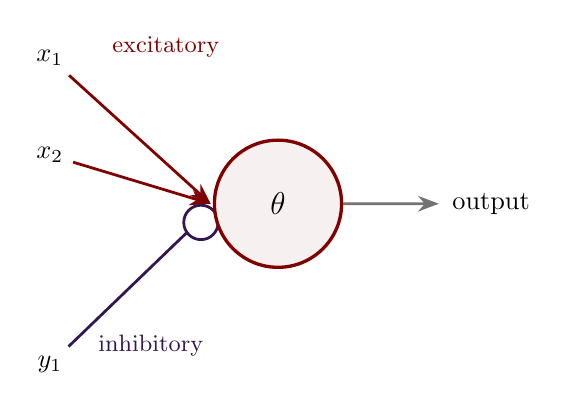
\begin{tikzpicture}[>=Stealth, line width=0.8pt,
          scale=0.95, transform shape, font=\normalsize]
        \foreach \i/\y in {1/2.2, 2/0.9}{
          \node (x\i) at (0,\y) {$x_{\i}$};
          \draw[->, dpc, line width=1.0pt] (x\i) -- (2.15,0.25);
        }
        \node (y1) at (0,-1.9) {$y_{1}$};
        \draw[shc, line width=1.0pt] (y1) -- (1.92,-0.05);
        \node[circle, draw=shc, fill=white, line width=1.0pt,
              minimum size=4.6mm, inner sep=0pt] at (2.02,0.0) {};
        \node[circle, draw=dpc, fill=dpc!6, line width=1.2pt,
              minimum size=17mm, inner sep=0pt] (u) at (3.05,0.25)
              {\large$\theta$};
        \draw[->, black!55, line width=1.0pt] (u) -- (5.2,0.25);
        \node[right, font=\normalsize] at (5.25,0.25) {output};
        \node[font=\small, dpc] at (1.55,2.35) {excitatory};
        \node[font=\small, shc] at (1.35,-1.65) {inhibitory};
      \end{tikzpicture}
    \end{column}
    \hfill
    \begin{column}{0.48\textwidth}
      \vspace{0.3em}
      \begin{itemize}\setlength{\itemsep}{2pt}
        \item Inputs and output are \alert{binary}
              ($0$ or $1$); edges are unweighted
        \item Edges are \alert{excitatory} or
              \alert{inhibitory} (small circle)
        \item Each unit has a threshold $\theta$
              \hfill{\scriptsize Rojas (1996), \S2.1.2}
      \end{itemize}
    \end{column}
  \end{columns}
  \biomodel{excitatory / inhibitory synapses}
           {excitatory / inhibitory edges into a threshold
            unit}
\end{frame}

\begin{frame}{The firing rule}
  A unit receives $x_1,\dots,x_n$ on $n$ excitatory edges and
  $y_1,\dots,y_m$ on $m$ inhibitory edges
 
  \vspace{0.1em}
  \begin{itemize}\setlength{\itemsep}{1pt}
    \item If $m\ge 1$ and \alert{any} inhibitory signal
          $y_j = 1$: the unit is \alert{inhibited},
          output $=0$
    \item Otherwise compute $z = x_1+\cdots+x_n$ and compare
          with $\theta$:
          $\quad\text{output}=1$ if $z\ge\theta$, else $0$
    \item With no inhibition, the unit acts as a
          \alert{threshold gate}
  \end{itemize}
  \biomodel{fire iff input exceeds threshold; inhibition can
            veto}
           {output $1$ iff $z\ge\theta$; any active inhibitor
            forces $0$}
\end{frame}

\begin{frame}{The activation is a step function}
  \centering
  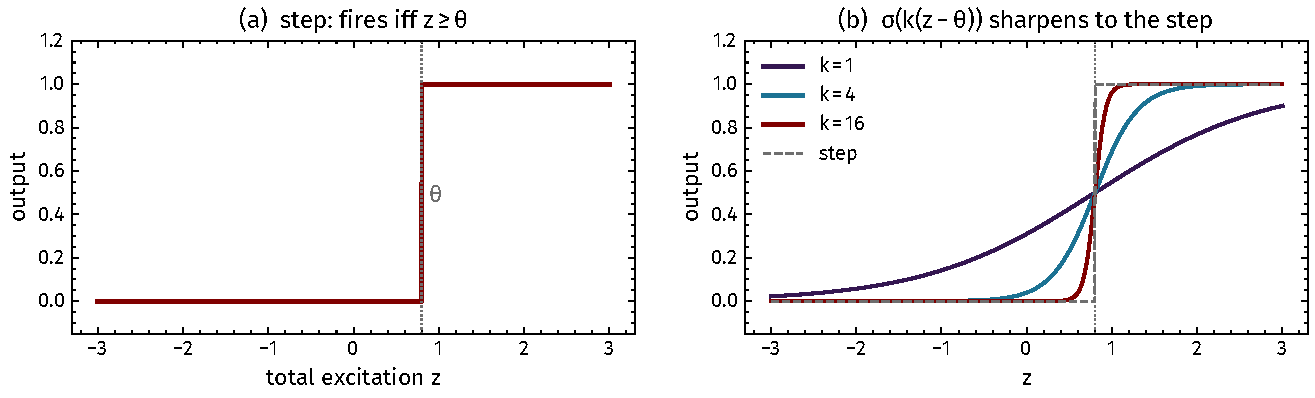
\includegraphics[height=0.42\textheight]{step_activation}
  \\[0.15em]
  \figsource{(a) the step (Heaviside) activation: the output
  jumps discontinuously from $0$ to $1$ at $z=\theta$.
  (b) a logistic $\sigma(k(z-\theta))$ for increasing
  sharpness $k$ --- as $k$ grows it converges to the step.}
  \vspace{0.1em}
  \begin{itemize}\setlength{\itemsep}{0pt}
    \item The hard threshold mirrors the neuron's
          all-or-nothing spike; the smooth versions in (b)
          return in Classes 5--6, where we need derivatives
  \end{itemize}
\end{frame}

% =====================================================================
\section{Computing with Threshold Logic}
% =====================================================================

\begin{frame}{Boolean functions from threshold gates}
  \begin{columns}[T, onlytextwidth]
    \begin{column}{0.46\textwidth}
      \centering
      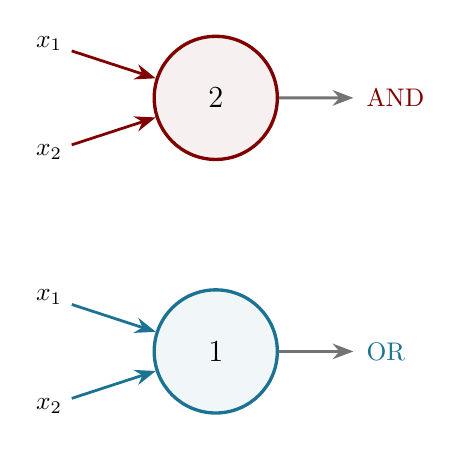
\begin{tikzpicture}[>=Stealth, line width=0.9pt,
          scale=0.92, transform shape, font=\normalsize]
        % AND
        \node (a1) at (0,2.0) {$x_1$};
        \node (a2) at (0,0.5) {$x_2$};
        \node[circle, draw=dpc, fill=dpc!6, line width=1.2pt,
              minimum size=17mm, inner sep=0pt] (ga) at (2.3,1.25)
              {\large$2$};
        \draw[->, dpc, line width=1.0pt] (a1)--(ga);
        \draw[->, dpc, line width=1.0pt] (a2)--(ga);
        \draw[->, black!55, line width=1.0pt] (ga)--(4.2,1.25);
        \node[right, font=\normalsize, dpc] at (4.25,1.25) {AND};
        % OR
        \node (b1) at (0,-1.5) {$x_1$};
        \node (b2) at (0,-3.0) {$x_2$};
        \node[circle, draw=tealc, fill=tealc!6, line width=1.2pt,
              minimum size=17mm, inner sep=0pt] (gb) at (2.3,-2.25)
              {\large$1$};
        \draw[->, tealc, line width=1.0pt] (b1)--(gb);
        \draw[->, tealc, line width=1.0pt] (b2)--(gb);
        \draw[->, black!55, line width=1.0pt] (gb)--(4.2,-2.25);
        \node[right, font=\normalsize, tealc] at (4.25,-2.25) {OR};
      \end{tikzpicture}
    \end{column}
    \hfill
    \begin{column}{0.50\textwidth}
      \vspace{0.2em}
      {\small Two binary inputs, $1=$ \emph{true}:}
      \begin{itemize}\setlength{\itemsep}{2pt}
        \item \alert{AND}: threshold $\theta=2$ --- fires only
              if \emph{both} inputs are $1$
        \item \alert{OR}: threshold $\theta=1$ --- fires if
              \emph{either} input is $1$
        \item \alert{NOT}: one inhibitory edge and
              $\theta = 0$
      \end{itemize}
      {\small A single unit already computes the fundamental
      logic gates.}
    \end{column}
  \end{columns}
  \biomodel{a neuron as a coincidence detector}
           {a threshold gate computing AND / OR}
\end{frame}

\begin{frame}{The same gates, drawn in input space}
  \centering
  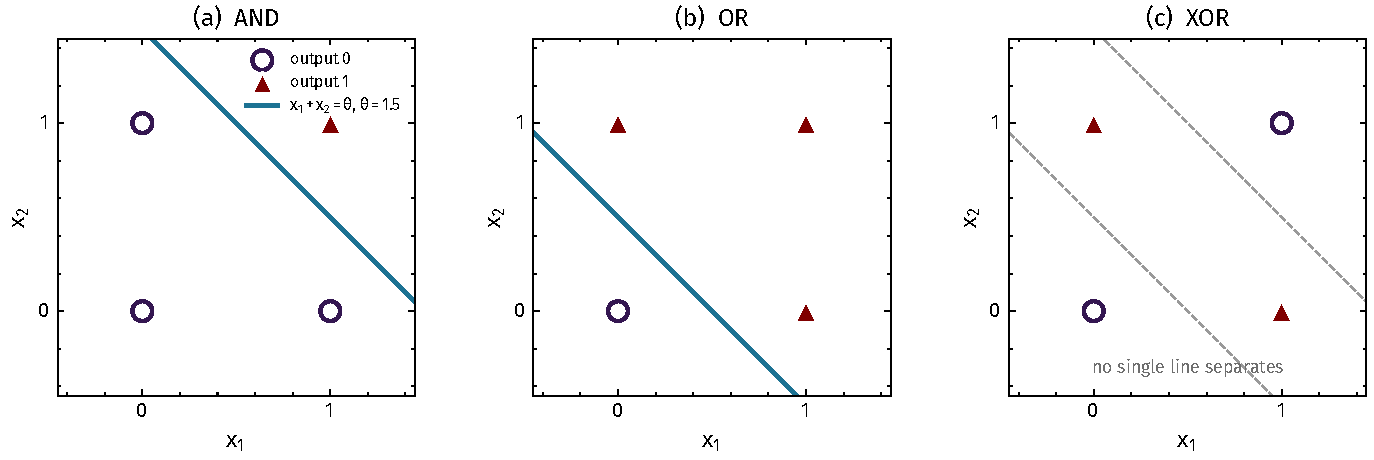
\includegraphics[height=0.40\textheight]{logic_2d}
  \\[0.15em]
  \figsource{The four input pairs of a two-input Boolean
  function. Triangles output $1$, open circles output $0$.
  (a) AND and (b) OR are each split by the line
  $x_1+x_2=\theta$ --- only $\theta$ differs.
  (c) XOR cannot be split by any straight line.}
  \biomodel{a neuron responds to a region of stimulus space}
           {a unit responds to a \alert{half-plane} of inputs}
\end{frame}

\begin{frame}{Threshold logic is expressive}
  \begin{itemize}
    \item A single unit can compute AND or OR of \alert{$n$
          arguments} --- just set $\theta = n$ (AND) or
          $\theta = 1$ (OR)
    \item Negation needs an \alert{inhibitory} edge: a unit
          with $\theta = 0$ and one inhibitory input computes
          NOT
    \item With AND, OR, and NOT available, threshold-logic
          networks can compute \alert{any Boolean function}
          \hfill{\scriptsize Rojas (1996), \S2.2}
  \end{itemize}
  \vspace{0.3em}
  \begin{redhighlight}
    But how expressive is a \emph{single} unit? The answer is
    geometric.
  \end{redhighlight}
\end{frame}

\begin{frame}{Any Boolean function, by construction}
  A logical function is a \alert{table}: for each input
  vector, a $0$ or a $1$. To build a network for it
  (Rojas, 1996, \S2.2.3):
  \vspace{0.2em}
  \begin{enumerate}\setlength{\itemsep}{2pt}
    \item For every input row that should output $1$, use one
          unit as a \alert{decoder} --- it fires \emph{only}
          for that exact vector
    \item A decoder for $(1,0,1)$: excitatory edges from the
          $1$-bits, inhibitory from the $0$-bits, threshold
          $=$ number of $1$-bits
    \item Feed all decoders into a single \alert{OR} unit
  \end{enumerate}
  \vspace{0.3em}
  \begin{redhighlight}
    Two layers of threshold units suffice for \emph{any}
    Boolean function --- expressive power is not the problem.
  \end{redhighlight}
\end{frame}

% =====================================================================
\section{Geometry: Linear Separability}
% =====================================================================

\begin{frame}{A unit splits input space into half-spaces}
  \begin{columns}[T, onlytextwidth]
    \begin{column}{0.54\textwidth}
      \centering
      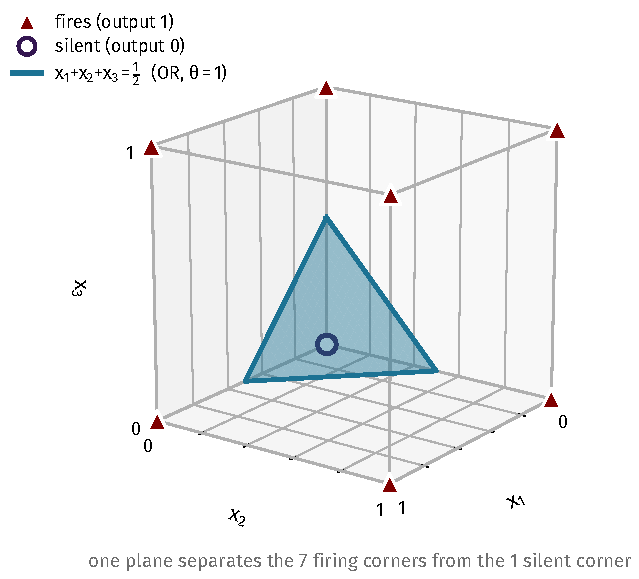
\includegraphics[height=0.52\textheight]{cube_or}
    \end{column}
    \hfill
    \begin{column}{0.42\textwidth}
      \vspace{0.3em}
      {\small For three binary inputs and threshold $\theta$,
      the unit tests $x_1{+}x_2{+}x_3 \ge \theta$:}
      \begin{itemize}\setlength{\itemsep}{2pt}
        \item The equality $x_1{+}x_2{+}x_3=\theta$ is a
              \alert{separating plane}
        \item One side fires ($\blacktriangle$), the other
              does not ($\circ$)
        \item OR: only the all-zero vertex lies below the
              plane
      \end{itemize}
    \end{column}
  \end{columns}
  \biomodel{a neuron responds to a region of stimulus space}
           {a unit responds to a \emph{half-space} of inputs}
\end{frame}

\begin{frame}{Parallel planes, different thresholds}
  \begin{columns}[T, onlytextwidth]
    \begin{column}{0.54\textwidth}
      \centering
      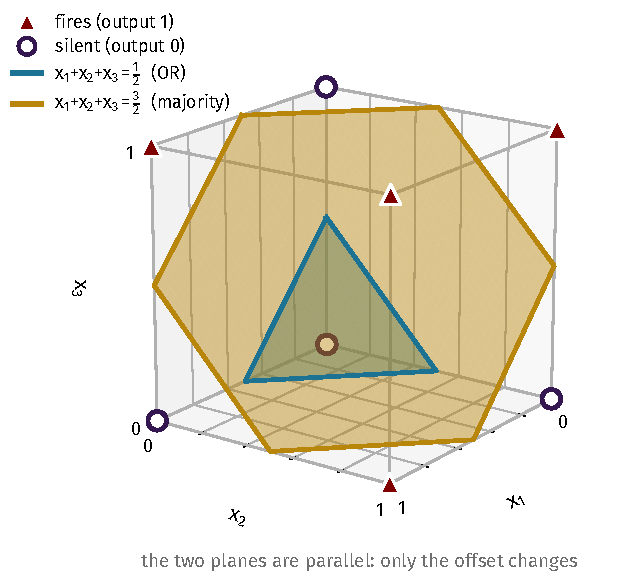
\includegraphics[height=0.52\textheight]{cube_majority}
    \end{column}
    \hfill
    \begin{column}{0.42\textwidth}
      \vspace{0.3em}
      \begin{itemize}\setlength{\itemsep}{2pt}
        \item \alert{OR}: plane at $\theta=1$
              (teal) --- fires unless all inputs are $0$
        \item \alert{Majority}: plane at $\theta=2$
              (amber) --- fires when at least two inputs
              are $1$
        \item With unit weights the planes stay
              \alert{parallel}
        \item \alert{Non-parallel} planes need
              \alert{weighted} edges --- the perceptron
              (Class 3)
      \end{itemize}
    \end{column}
  \end{columns}
  \figsource{Vertices show the majority function.}
\end{frame}

\begin{frame}{The one it cannot do: XOR}
  \begin{columns}[T, onlytextwidth]
    \begin{column}{0.42\textwidth}
      \centering
      \begin{tikzpicture}[line width=0.9pt, scale=1.7]
        \draw[->, black!55] (-0.25,0) -- (1.4,0)
          node[right,font=\scriptsize]{$x_1$};
        \draw[->, black!55] (0,-0.25) -- (0,1.4)
          node[above,font=\scriptsize]{$x_2$};
        \node[circle, draw=shc, fill=white, minimum size=4.6pt,
              inner sep=1.3pt, line width=0.9pt] at (0,0) {};
        \node[circle, draw=shc, fill=white, minimum size=4.6pt,
              inner sep=1.3pt, line width=0.9pt] at (1,1) {};
        \node[dpc, font=\small] at (0,1) {$\bm\blacktriangle$};
        \node[dpc, font=\small] at (1,0) {$\bm\blacktriangle$};
        \draw[mcMuted, dashed] (-0.15,0.65) -- (1.2,0.78);
        \draw[mcMuted, dashed] (0.42,-0.15) -- (0.63,1.25);
        \node[font=\scriptsize] at (-0.16,-0.16) {$0$};
        \node[font=\scriptsize] at (1.14,1.14) {$1$};
      \end{tikzpicture}
      \\[0.2em]
      \figsource{$\blacktriangle$: XOR $=1$; \
      $\circ$: XOR $=0$.}
    \end{column}
    \hfill
    \begin{column}{0.54\textwidth}
      \vspace{0.3em}
      \begin{itemize}\setlength{\itemsep}{2pt}
        \item XOR outputs $1$ when the inputs \alert{differ},
              $0$ when they agree
        \item The two $\blacktriangle$ sit on \alert{opposite
              corners} --- so do the two $\circ$
        \item \alert{No single straight line} can put both
              $\blacktriangle$ on one side and both $\circ$ on
              the other
        \item XOR is \alert{not linearly separable} --- a wall
              a single unit cannot climb
      \end{itemize}
    \end{column}
  \end{columns}
\end{frame}

\begin{frame}{How rare is linear separability?}
  \centering
  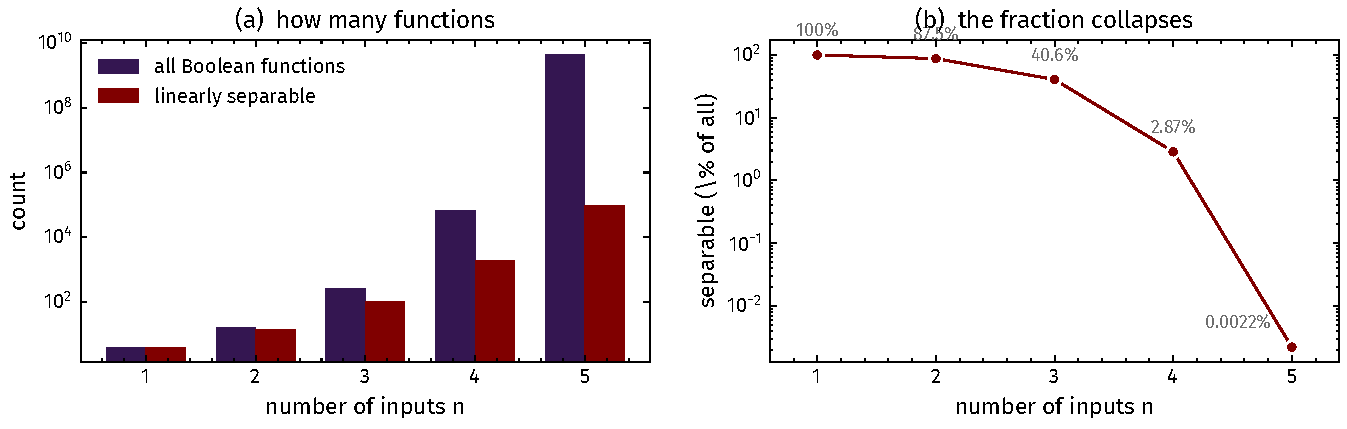
\includegraphics[height=0.42\textheight]{separable_fraction}
  \\[0.15em]
  \figsource{(a) of all $2^{2^n}$ Boolean functions of $n$
  inputs, only a small number are linearly separable
  ($4, 14, 104, 1882, 94572$ for $n=1\ldots5$).
  (b) as a percentage, that share collapses --- by $n=5$ it is
  about $0.002\%$.}
  \vspace{0.1em}
  \begin{itemize}\setlength{\itemsep}{0pt}
    \item XOR is not a curiosity: \alert{almost every} Boolean
          function is out of reach for a single unit
  \end{itemize}
\end{frame}

\begin{frame}{Linear separability --- and its limit}
  \begin{itemize}
    \item A single threshold unit computes exactly the
          \alert{linearly separable} functions: those whose
          $1$- and $0$-inputs can be split by a hyperplane
    \item AND, OR, majority --- all linearly separable
    \item XOR is not --- and as $n$ grows, almost nothing is
  \end{itemize}
  \vspace{0.3em}
  \begin{redhighlight}
    A single unit is a linear classifier. Escaping
    linear separability needs \alert{weights} (Class 3) and,
    ultimately, \alert{layers} (Classes 5--7).
  \end{redhighlight}
\end{frame}

\begin{frame}{Takeaways}
  \begin{enumerate}\setlength{\itemsep}{2pt}
    \item A neuron integrates weighted inputs and fires when a
          \alert{threshold} is crossed --- all-or-nothing
    \item The \alert{McCulloch--Pitts unit} keeps only this:
          binary inputs, a threshold, excitatory/inhibitory
          edges
    \item A single unit computes AND, OR, majority --- but
          only \alert{linearly separable} functions
    \item Geometrically it is a \alert{separating hyperplane};
          XOR already escapes it, and almost every function
          does as $n$ grows
  \end{enumerate}
  \vspace{0.3em}
  \begin{redhighlight}
    Next Topic: add \alert{weights} and a \alert{learning rule}
    --- the perceptron.
  \end{redhighlight}
\end{frame}

\begin{frame}{References}
  \footnotesize
  \begin{itemize}\setlength{\itemsep}{3pt}
    \item R.~Rojas. \textit{Neural Networks: A Systematic
          Introduction.} Springer, 1996. Chapters 1--2 ---
          biological motivation, threshold logic, geometric
          interpretation.
    \item W.~S.~McCulloch \& W.~Pitts (1943). ``A logical
          calculus of the ideas immanent in nervous
          activity.'' \textit{Bulletin of Mathematical
          Biophysics}, 5, 115--133.
    \item Counts of linearly separable Boolean functions:
          OEIS A000609.

  \end{itemize}
\end{frame}

% \begin{frame}[standout]
%   Questions?
% \end{frame}

\end{document}
